
図\ref{fig:pdr-remove-drift}の軌跡の問題点として初期進行方向の誤差がある.
初期進行方向が誤っていると,歩行者の実際の移動経路と大きく異なる軌跡になる.
この問題を解決するためには,適切な初期進行方向を見つけて軌跡全体を回転させる必要がある.
フロアマップ情報を元に軌跡を回転させる関数をListing\ref{lst:pdr-rotate}に示す.
引数として加速度DF,角度DF,表\ref{tab:map_dict}に示すフロアマップ情報DICT,フロア名,マップの1pxあたりの距離を受け取る.
内部の処理としては軌跡を回転させその時の水平垂直方向の割合を計算する.
軌跡における垂直成分と水平成分を可視化したものが図\ref{fig:color}である.
この割合が最も大きい回転角度をグリッドサーチを用いて探し最適な角度を見つける.
しかしこの処理だけでは適切な初期進行方向は絞り込めない.
割合が大きいものがあっても90度回転させるごとに水平垂直方向の割合が同一になる
ため4つの角度から適切な初期進行方向を見つける必要がある.
この絞り込みの処理としてマップ上の通行可能,不可能な座標の情報を利用する.
各回転角度での軌跡座標がマップ上で通行可能なポイントの数を計算し最も多いポイントを持つ回転角度を選択する.
この処理を適用した結果が図\ref{fig:pdr-rotate}である.
補正前と比べて軌跡の初期進行方向が正解軌跡に近づいている.

\begin{lstlisting}[caption={初期進行方向補正}, label=lst:pdr-rotate]
def rotate_trajectory_to
		_optimal_alignment_using_map(
    acc_df: pd.DataFrame,
    angle_df: pd.DataFrame,
    map_dict: dict[str, np.ndarray],
    floor_name: str,
    dx: float,
    dy: float,
    *,
    ground_truth_first_point: dict[Axis2D, float] | None = None,
) -> tuple[pd.DataFrame, pd.DataFrame]:
\end{lstlisting}

\begin{table}[ht]
	\centering
	\begin{tabular}{lll}
		\hline
		      & \textbf{データ型}       & \textbf{説明}             \\ \hline
		key   & \texttt{str}        & floorの名前                \\ \hline
		value & \texttt{np.ndarray} & \makecell{フロアマップの画像データ. \\各フロアのブール値の\\NumPy配列} \\ \hline
	\end{tabular}
	\caption{フロマップ DICT}
	\label{tab:map_dict}
\end{table}

\begin{figure}[ht]
	\centering
	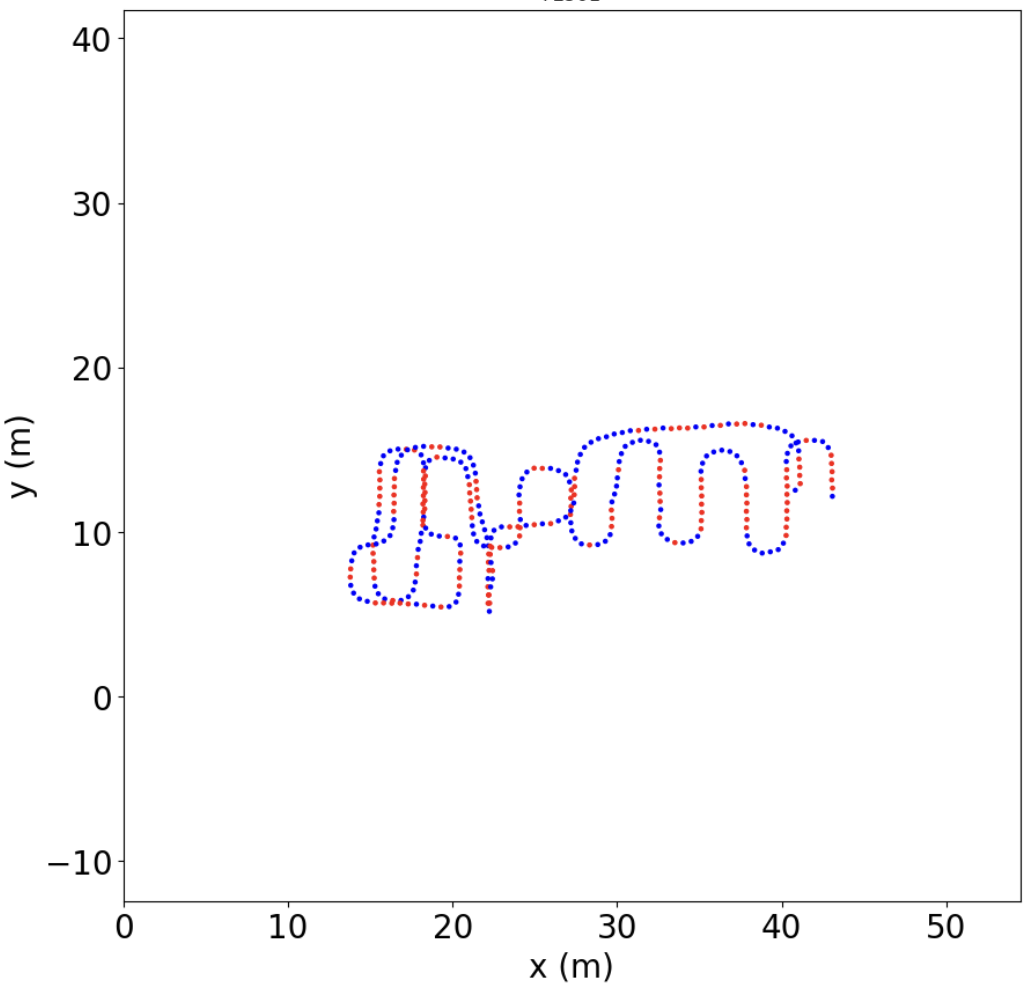
\includegraphics[width=80mm]{image/rb.jpg}
	\caption{垂直成分と水平成分の可視化}    \label{fig:color}
\end{figure}

\begin{figure}[ht]
	\centering
	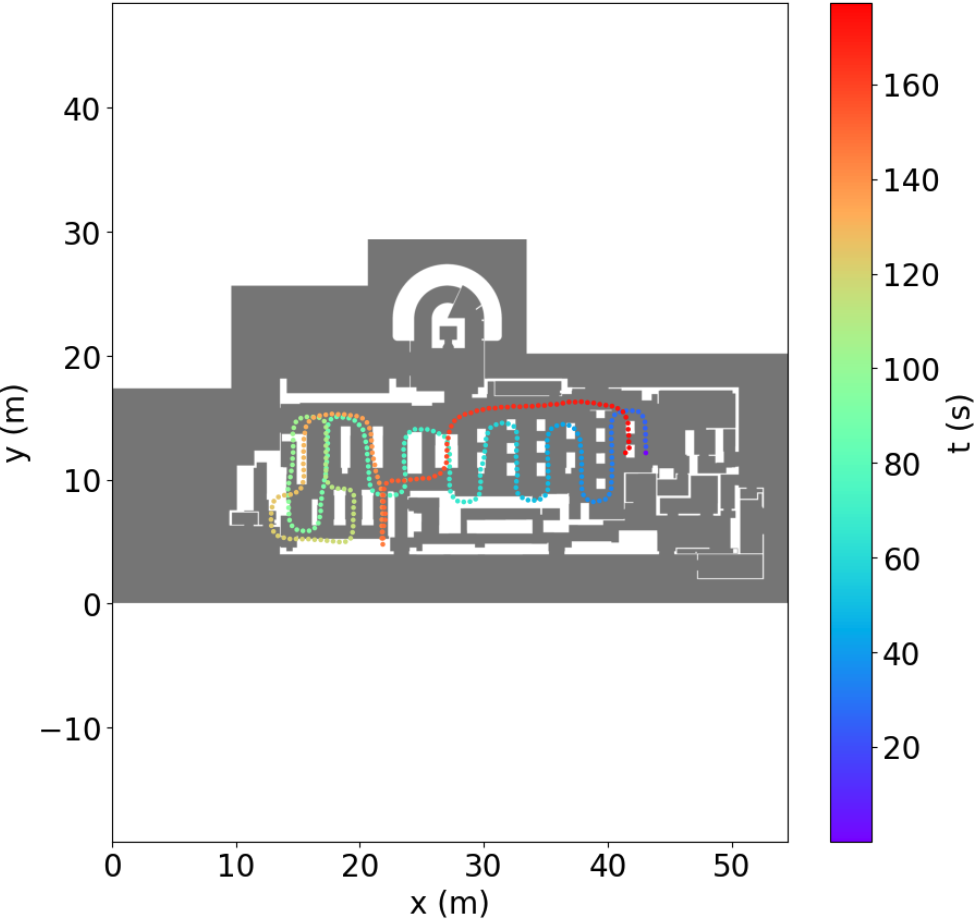
\includegraphics[width=80mm]{image/pdr-rotate.jpg}
	\caption{初期進行方向の補正後の軌跡}    \label{fig:pdr-rotate}
\end{figure}
